\chapter{Resultados}
\label{cap:resultados}

\pendiente{completar con las salidas del notebook ejecutado con \texttt{MODO\_RAPIDO = False}.}

\section{Entropía espectral (H5)}
\pendiente{sección 5 del notebook; figura~\ref{fig:h5}.}

\section{Caso convexo (H1)}
\pendiente{sección 6; figura~\ref{fig:convexo} y tabla de brechas.}

\section{Optimizadores}

\begin{figure}[ht]
\centering
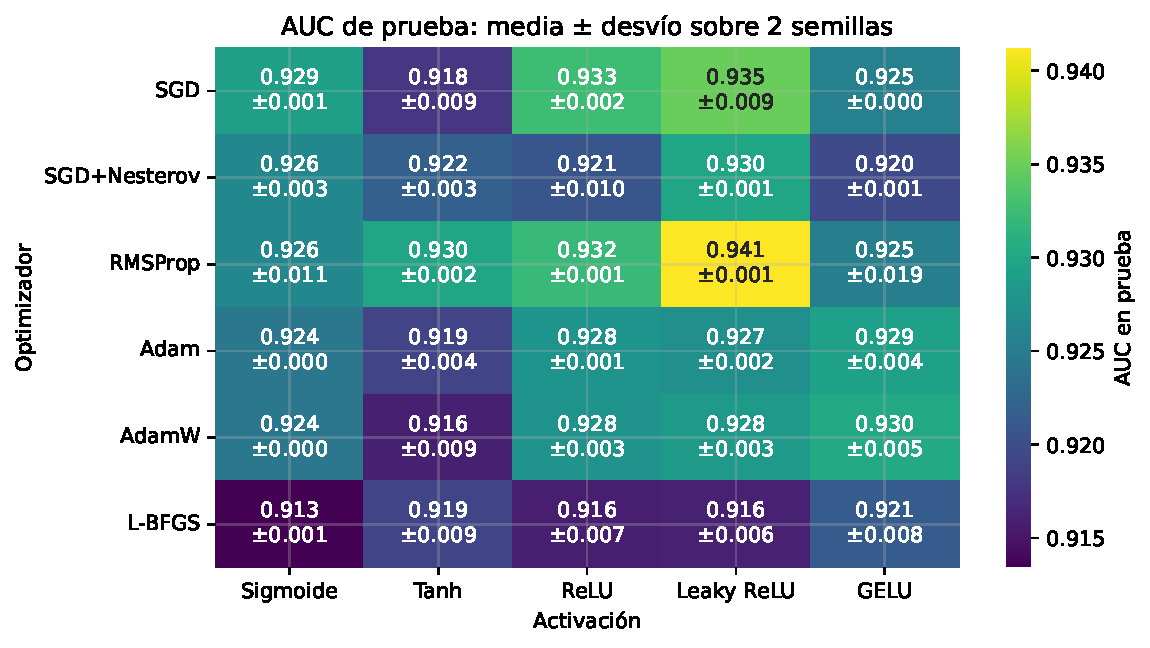
\includegraphics[width=0.8\linewidth]{grilla_heatmap_auc}
\caption{AUC de prueba (media $\pm$ desvío entre semillas) para cada combinación de optimizador y activación.}
\label{fig:heatmap}
\end{figure}

\pendiente{tasas elegidas, Friedman, rangos medios, Wilcoxon-Holm.}

\section{Funciones de activación e interacción (H2, H4)}

\begin{figure}[ht]
\centering
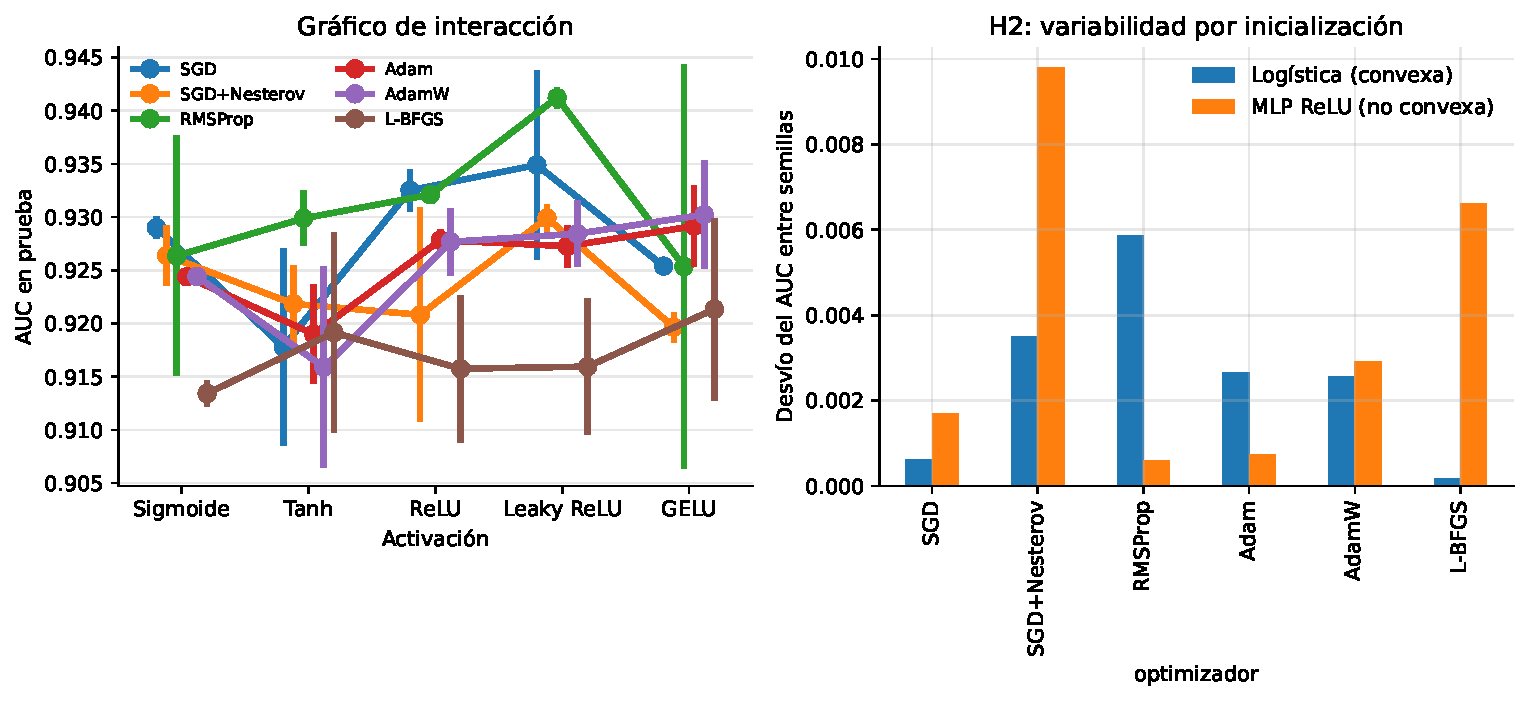
\includegraphics[width=\linewidth]{grilla_interaccion_variabilidad}
\caption{Izquierda: gráfico de interacción optimizador $\times$ activación. Derecha: desvío del AUC entre semillas en el caso convexo y no convexo.}
\label{fig:interaccion}
\end{figure}

\pendiente{ANOVA de dos factores y rango por optimizador.}

\section{Profundidad y desvanecimiento del gradiente (H3)}

\begin{figure}[ht]
\centering
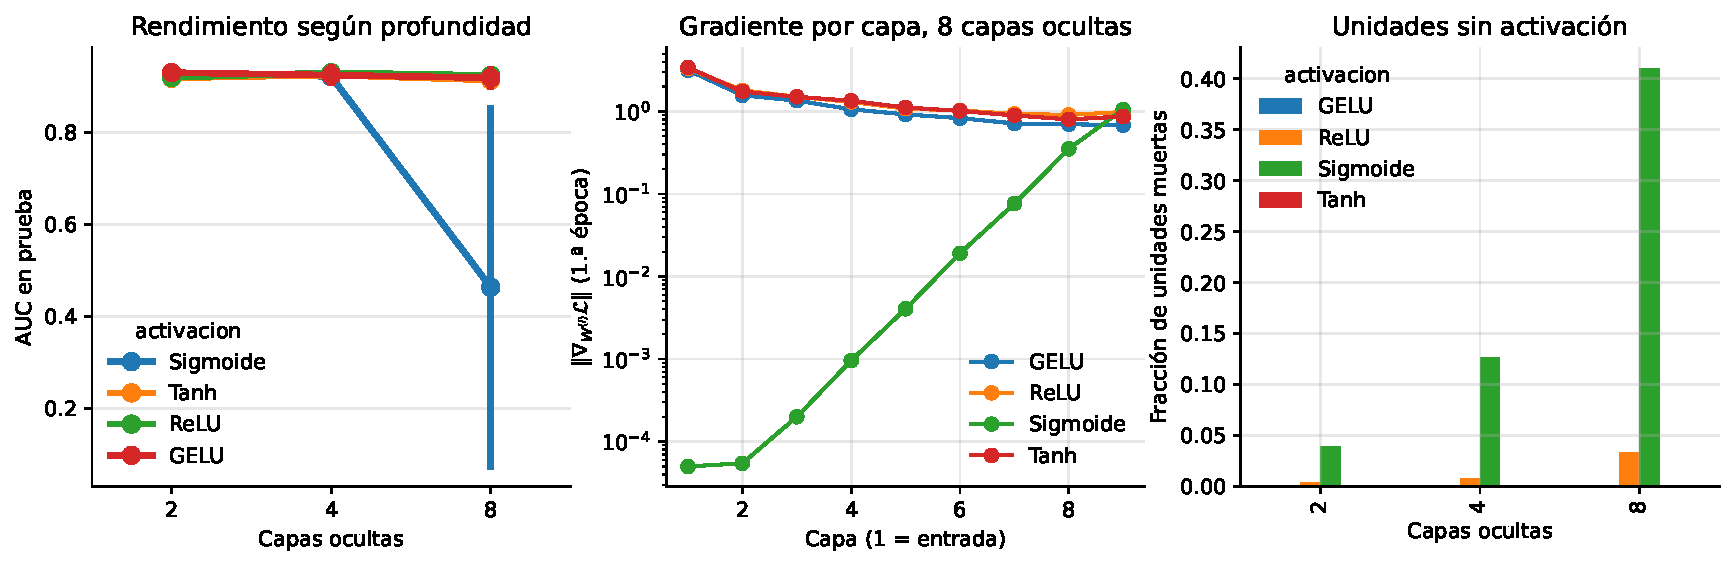
\includegraphics[width=\linewidth]{profundidad_gradientes}
\caption{AUC según profundidad, norma del gradiente por capa y fracción de unidades muertas.}
\label{fig:profundidad}
\end{figure}

\section{Evaluación del mejor modelo}

\begin{figure}[ht]
\centering
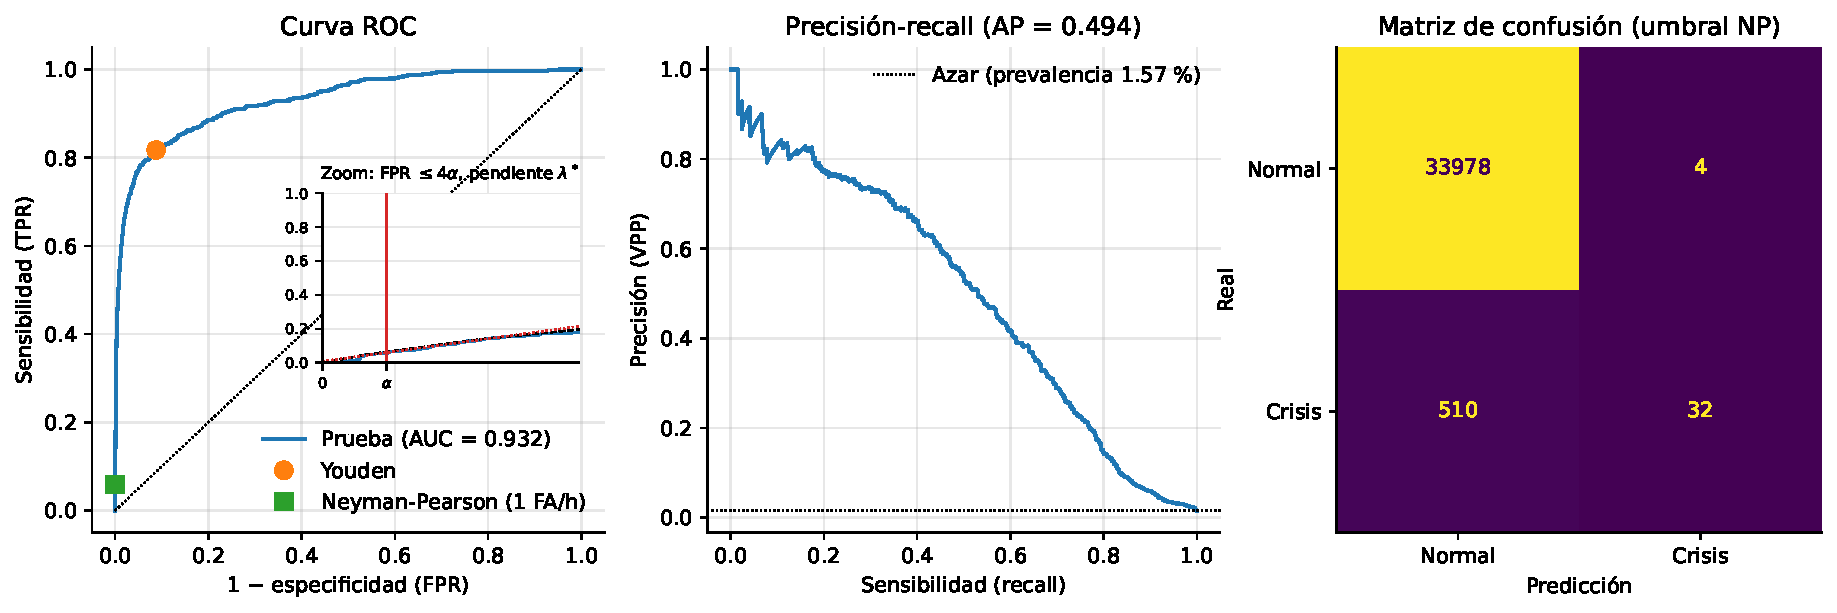
\includegraphics[width=\linewidth]{evaluacion_final}
\caption{Curva ROC (con el detalle de la región $\FPR\le 4\alpha$ y la pendiente $\lambda^\star$), curva precisión-recall y matriz de confusión con el umbral de Neyman-Pearson.}
\label{fig:evaluacion}
\end{figure}

\pendiente{tabla Youden vs. Neyman-Pearson; métricas por sujeto y por evento.}

\section{Sobreajuste}

\begin{figure}[ht]
\centering
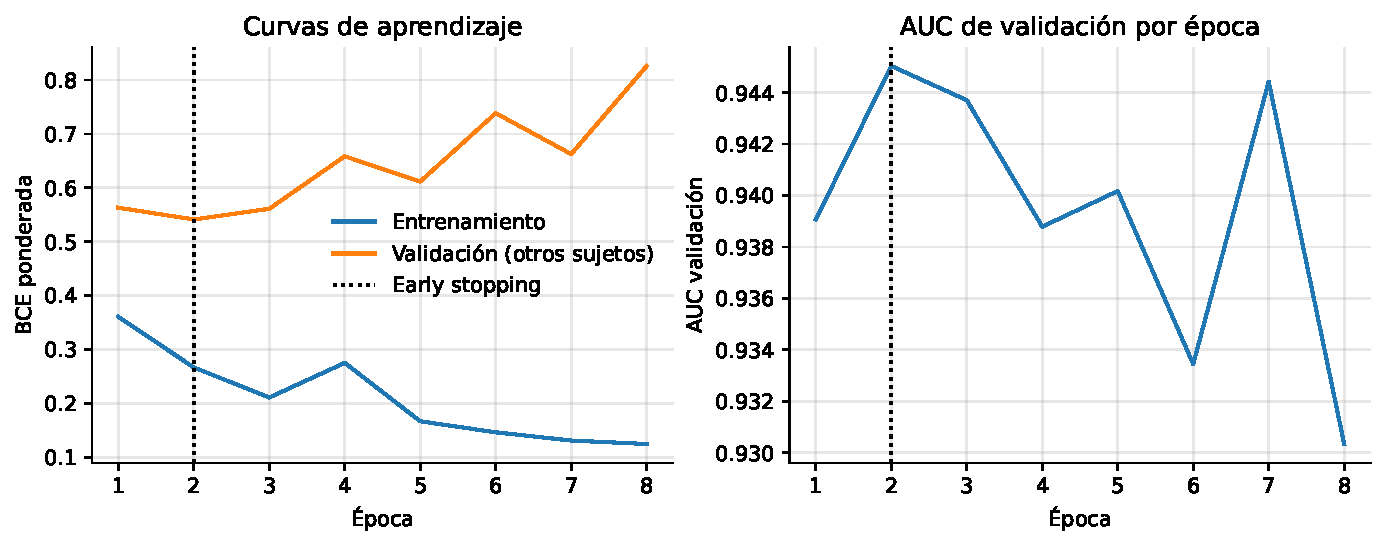
\includegraphics[width=\linewidth]{sobreajuste_curvas}
\caption{Curvas de pérdida y AUC de validación del mejor modelo.}
\label{fig:sobreajuste}
\end{figure}
